\section{Stoppages}

Stoppage represents another concept required for Transporter project users. Stoppage is a small movement of machine during large time on small territory. The vehicle can do some electricity supply repairing work or just stay on night stoppage at its base. It can also be located at some illegal places for a long time and that fact is requred to be captured for Transporter analysts.

It is very convenient to show the actual stoppages not only in tabular format but on the map. It gives an ability to analyse the common places at which the vehicle stops or whether the some group of vehicles were at base last night.

As the first example all stoppages of some concrete vehicle for 20 days has been shown (figure~\ref{fig:21}). As in all other places of the program, the large number of nodes groups to clusters. It gives an ability to conveniently zoom by clicking on the cluster. At the first time after Run action all stoppages are fitted to the bounds of the screen.

\begin{figure}[H]
\centering
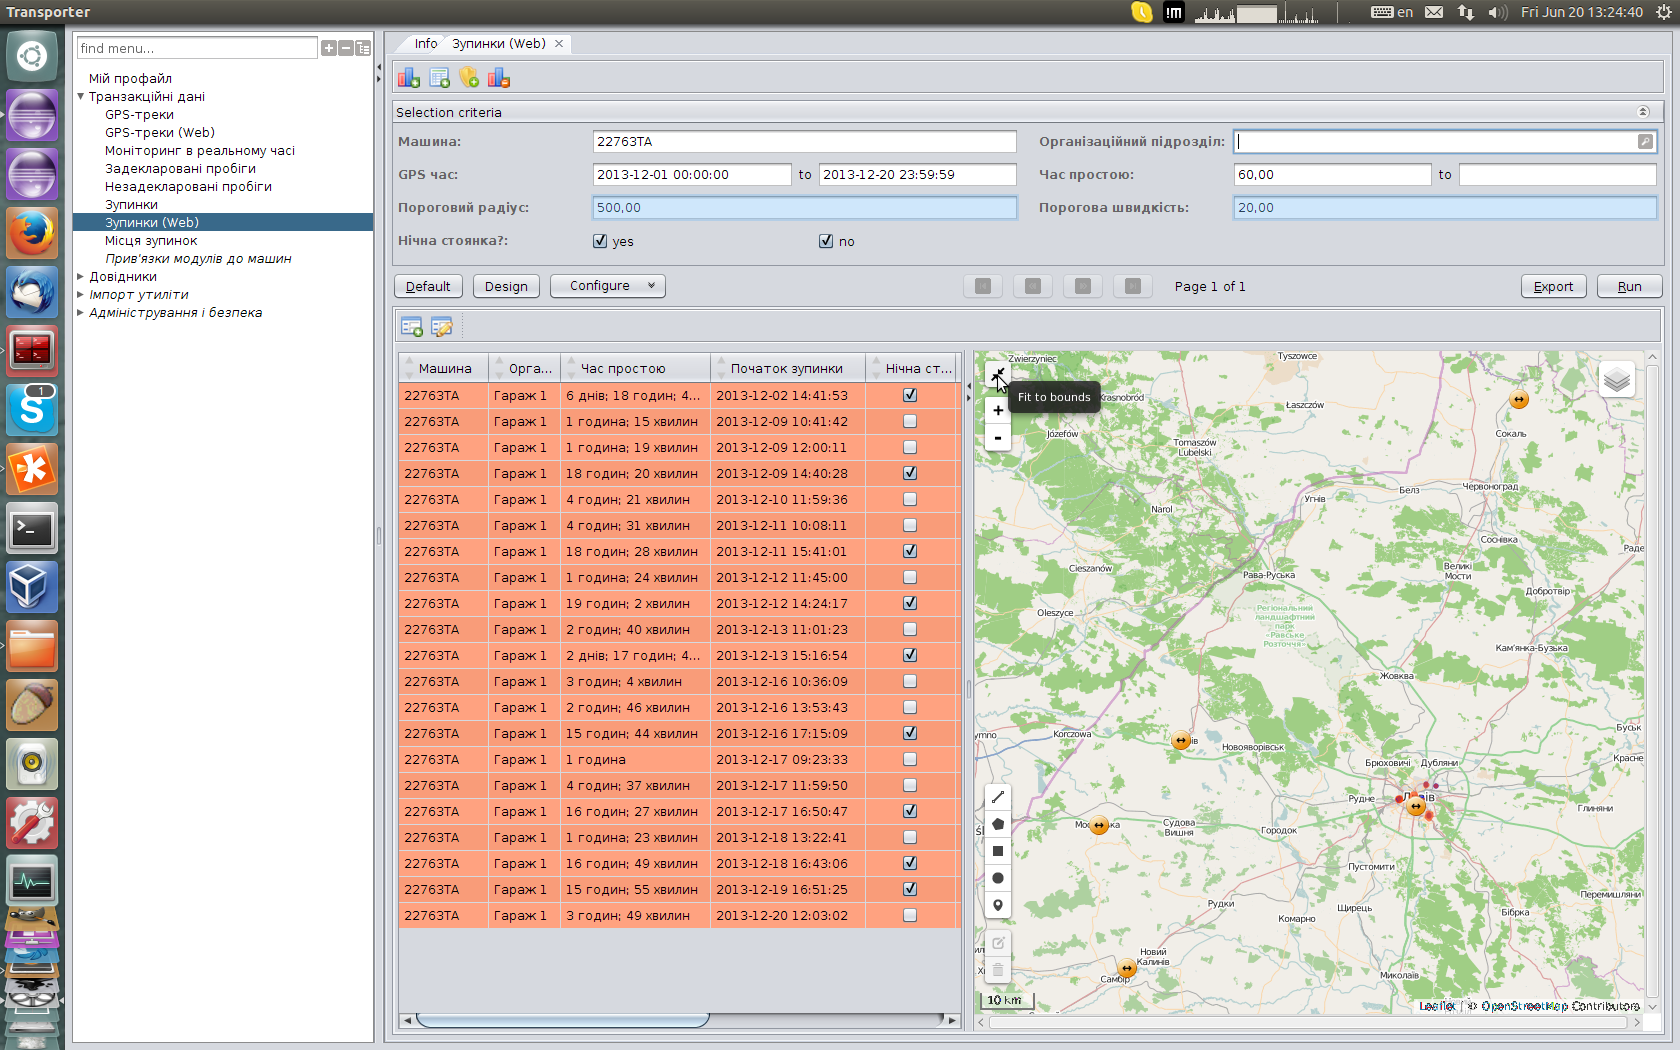
\includegraphics[width=\linewidth]{chapters/03-stoppages/images/21-all-stoppages-using-fit-to-bounds-button.png}
\caption{All stoppages has been fitted to the bounds using the button}\label{fig:21}
\end{figure}

\newpage
We can zoom to concrete stoppages of the vehicle near Lviv location by clicking on appropriate cluster (figure~\ref{fig:22}). The region polygon is shown when  the cluster is hovered (this behaviour is consistent with the behaviour of all other GIS views).

\begin{figure}[H]
\centering
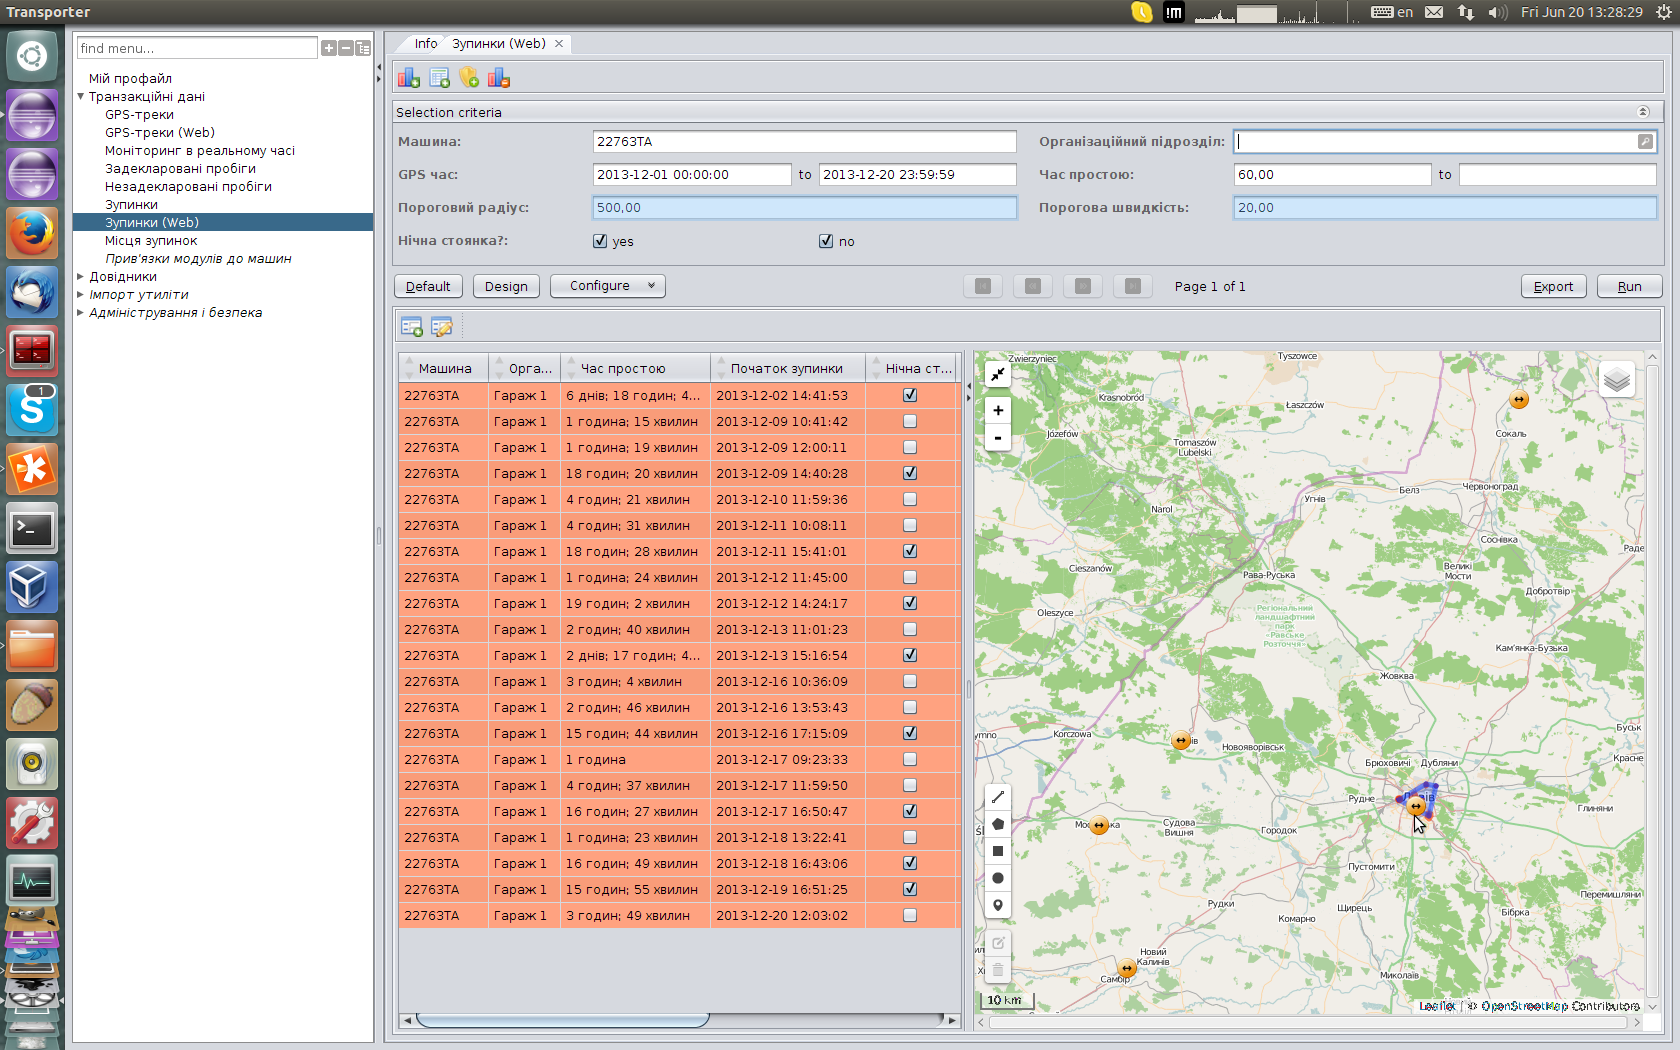
\includegraphics[width=\linewidth]{chapters/03-stoppages/images/22-part-of-stoppages-zooming-by-clicking-cluster-near-lviv.png}
\caption{Zooming by clicking the cluster near Lviv}\label{fig:22}
\end{figure}

\newpage
The part of stoppages are seen as the circular areas at which some small track movements appear (figure~\ref{fig:23}). The threshould radius can be configured using the selection criteria (however it is recommended for Transporter analysts to use 500 meters as optimal value). There is also an ability to filter by stoppage duration (for example, we can find the stoppages with duration longer than 1 hour) and to distinguish night stoppages from regular ones.

\begin{figure}[H]
\centering
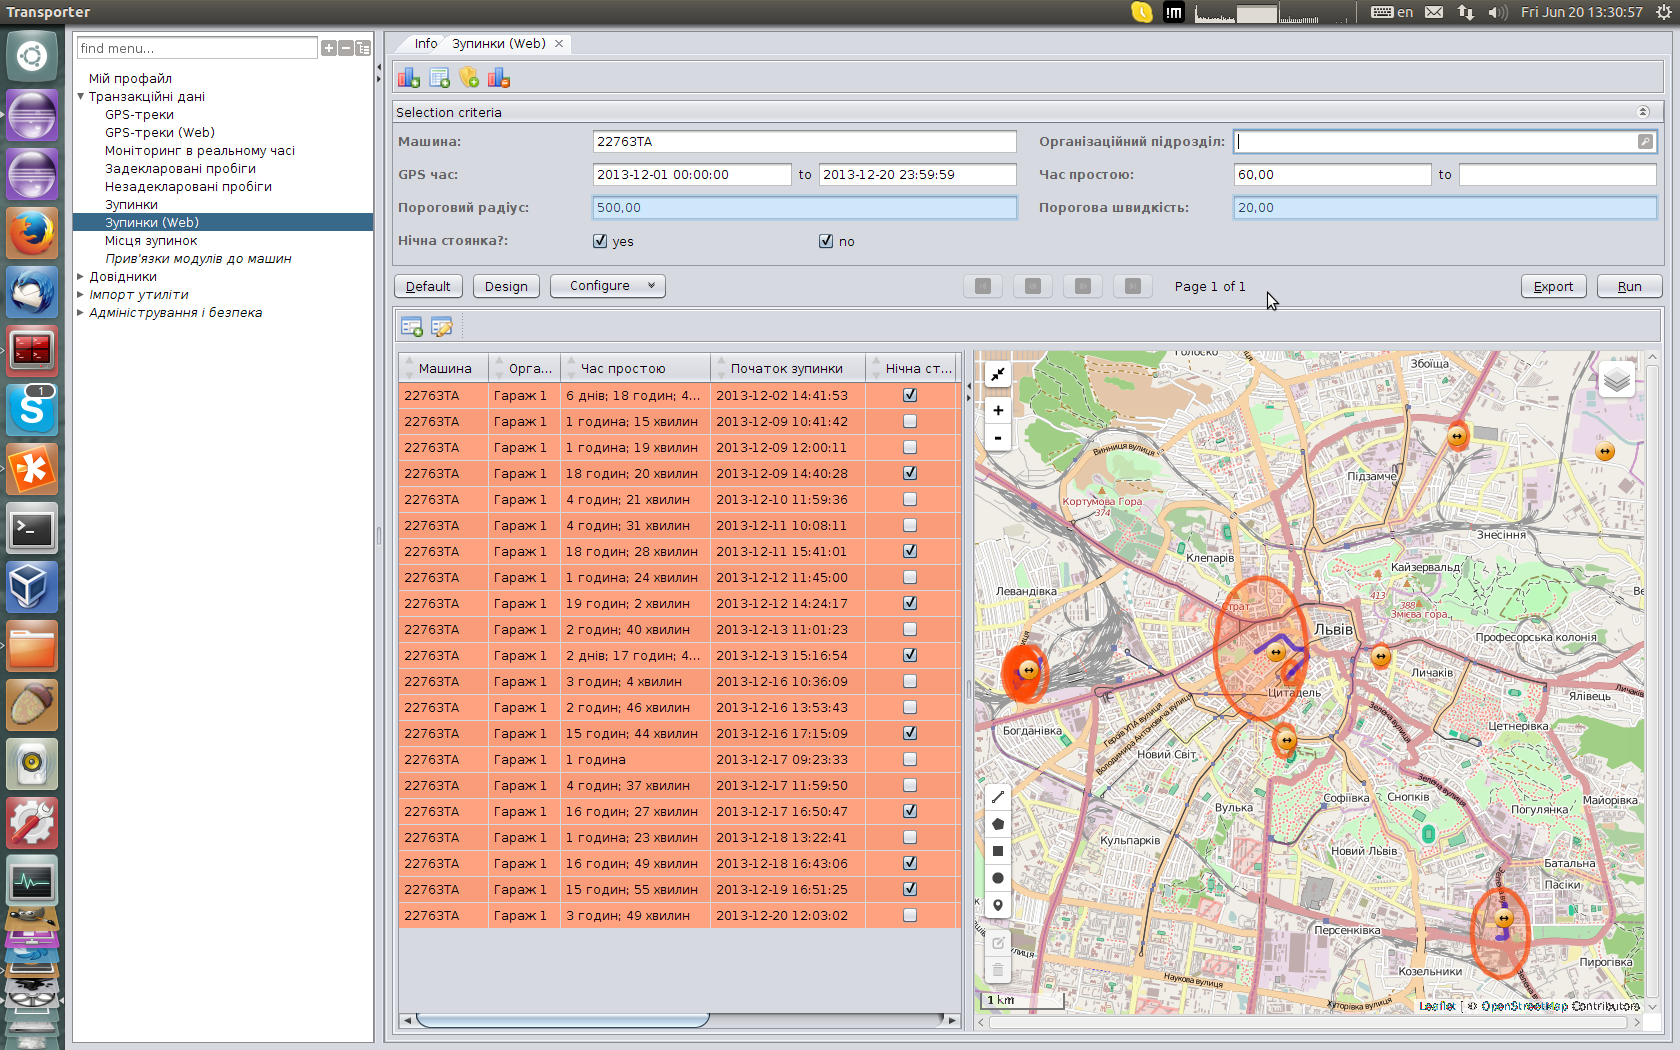
\includegraphics[width=\linewidth]{chapters/03-stoppages/images/23-part-of-stoppages-zoomed-in.png}
\caption{The part of stoppages zoomed in}\label{fig:23}
\end{figure}

\newpage 
The user can zoom to the base location of vehicles to see the stoppages of the vehicle at its base. As the circular areas are partially transparent, there can be seen multiple stoppages at the same place (figure~\ref{fig:24}). The detailed popup message has also been shown after stoppage selection. The popup message consists of all information that is shown in the grid row (all result-set properties that were chosen for entity centre are used in that case).

\begin{figure}[H]
\centering
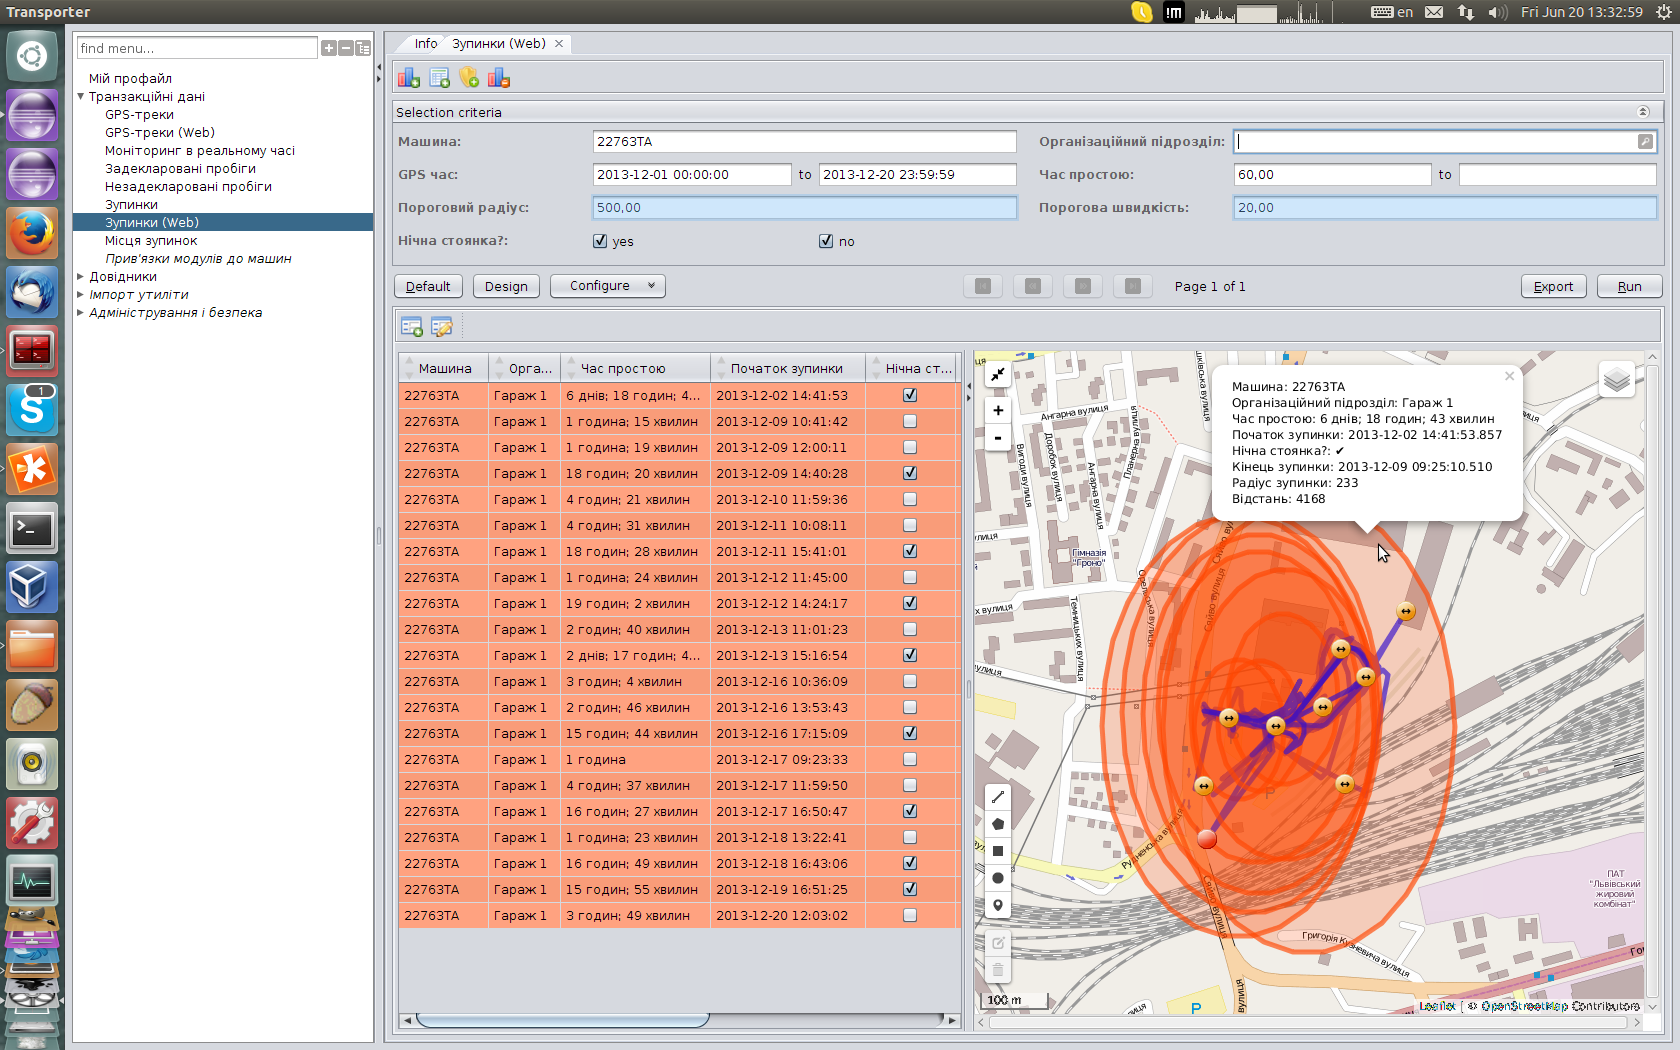
\includegraphics[width=\linewidth]{chapters/03-stoppages/images/24-a-plenty-of-night-stoppages-in-the-same-place-with-one-selected-popup-details.png}
\caption{A plenty of stoppages in the same place with one selected stoppage}\label{fig:24}
\end{figure}

\newpage
The detailed analysis of the stoppage can be performed directly in stoppage report by exploring the GPS-track details (figure~\ref{fig:25}). Full-featured GPS-track is ready with all GPS-messages and track polyline. There is no need to use separate ``GPS-tracks'' feature of the application.

\begin{figure}[H]
\centering
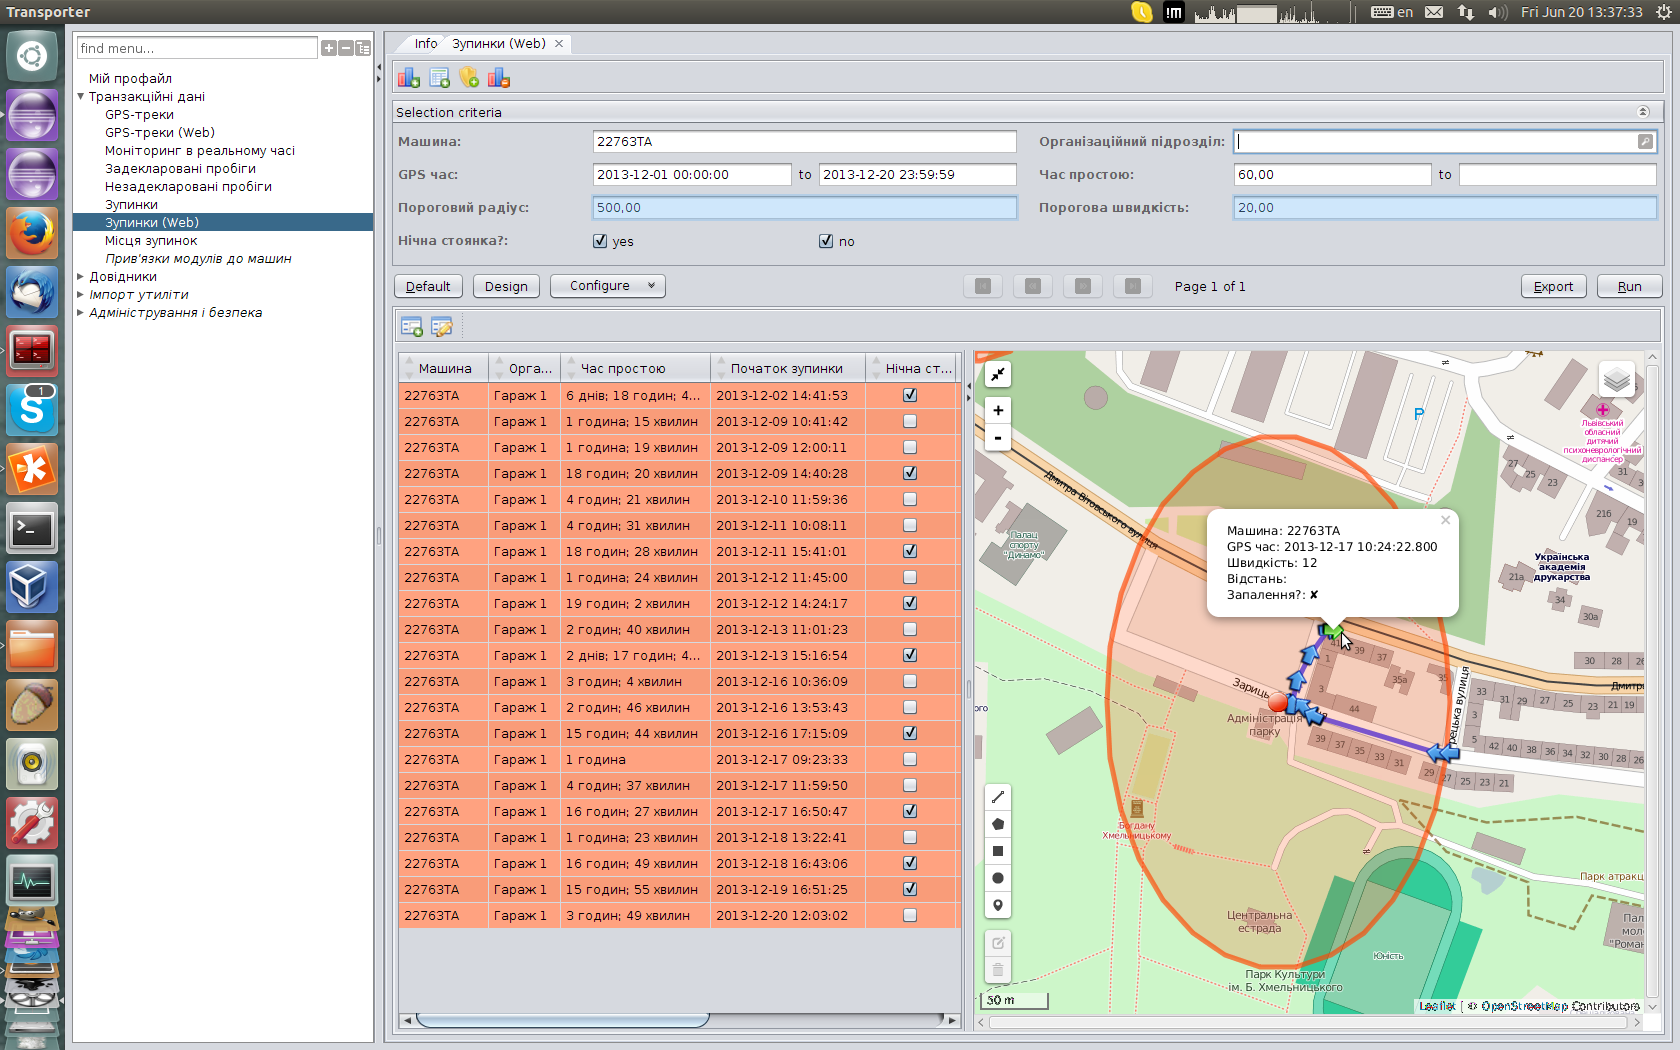
\includegraphics[width=\linewidth]{chapters/03-stoppages/images/25-detailed-stoppage-analysis-by-its-messages.png}
\caption{Detailed stoppage analysis by its GPS-messages}\label{fig:25}
\end{figure}

\newpage
The analyst can filter by the property ``Is Night Stoppage'' when he needs to determine whether the vehicle was at base every night at some period (figure~\ref{fig:26}). In this case all night stoppages are visually at the same place near the base. It means that no illegal night stoppages have been performed.

\begin{figure}[H]
\centering
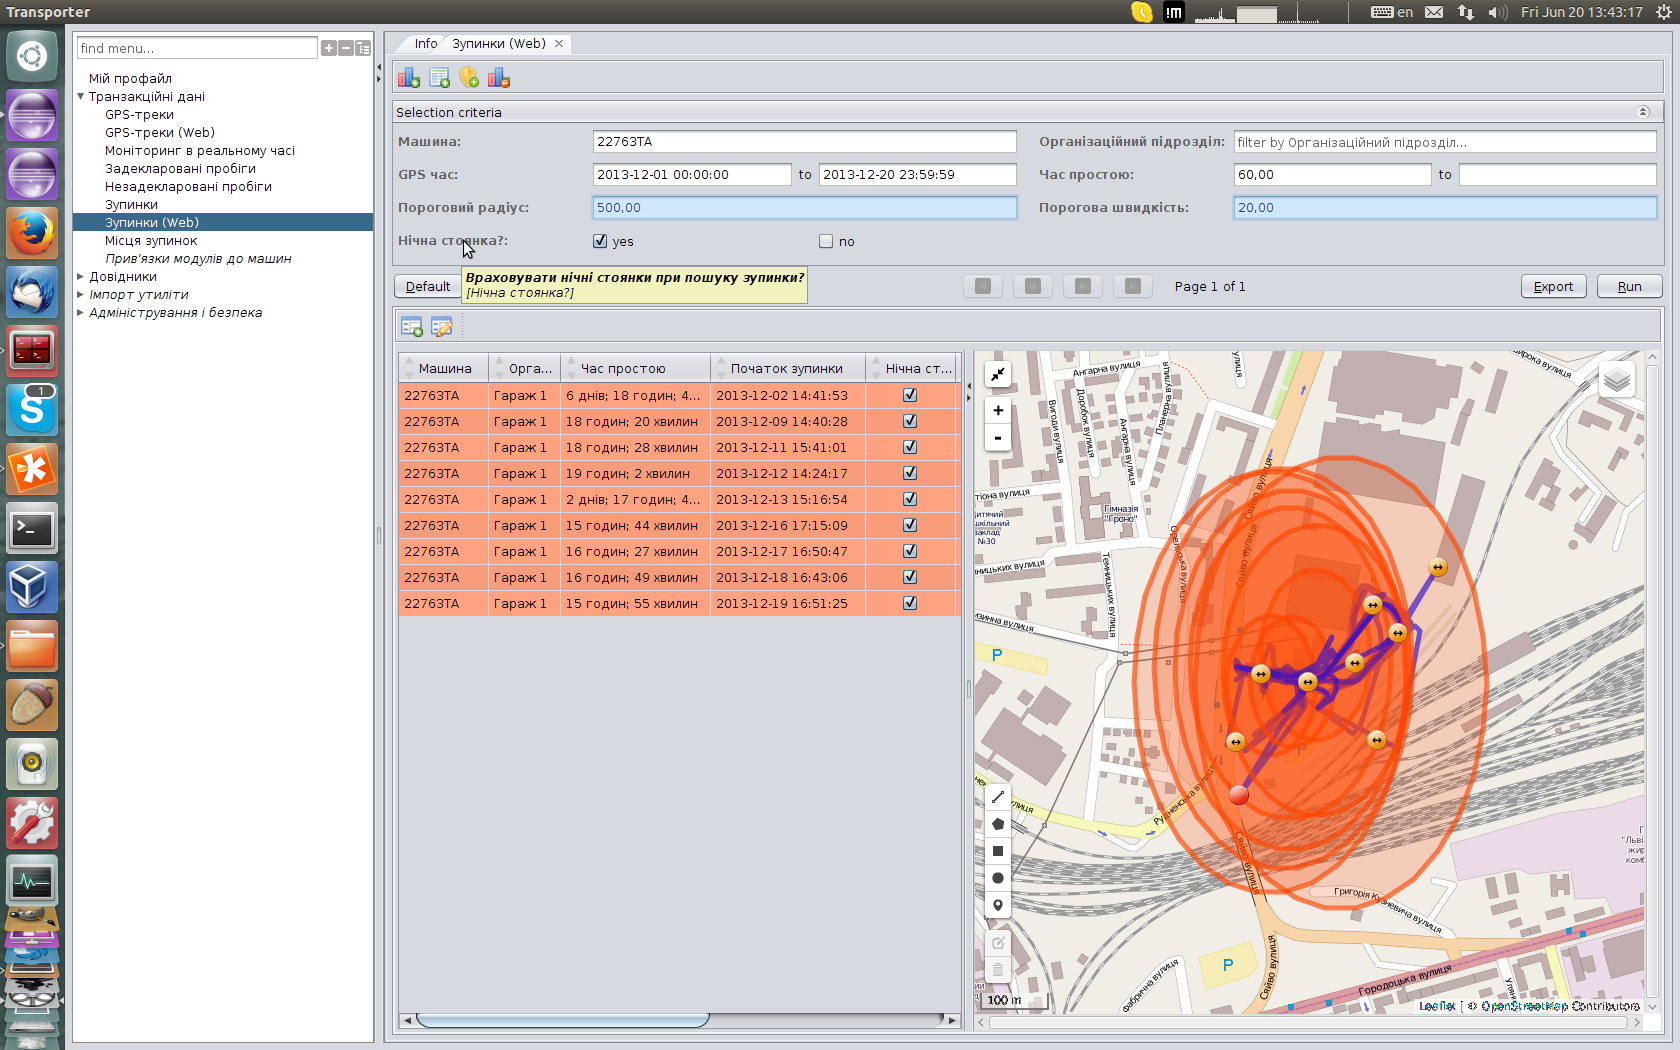
\includegraphics[width=\linewidth]{chapters/03-stoppages/images/26-determining-whether-machine-has-nightstopped-at-base-in-particular-period-of-time.png}
\caption{Determining whether machine has ``nightstopped'' at base in particular period of time}\label{fig:26}
\end{figure}

\newpage
A more fine-grained analysis can be performed when the analyst decreases the lower bound of stoppage duration. As the result we can see smaller stoppages with smaller durations, but no less than 15 minutes (figure~\ref{fig:27}).

As the additional requirement Transporter users suggest to provide the ability to filter stoppages by location. In this case, the previously developed support of complex Geo-zones can be reused (and ``Geo-coding'' feature is promising to be useful too).

\begin{figure}[H]
\centering
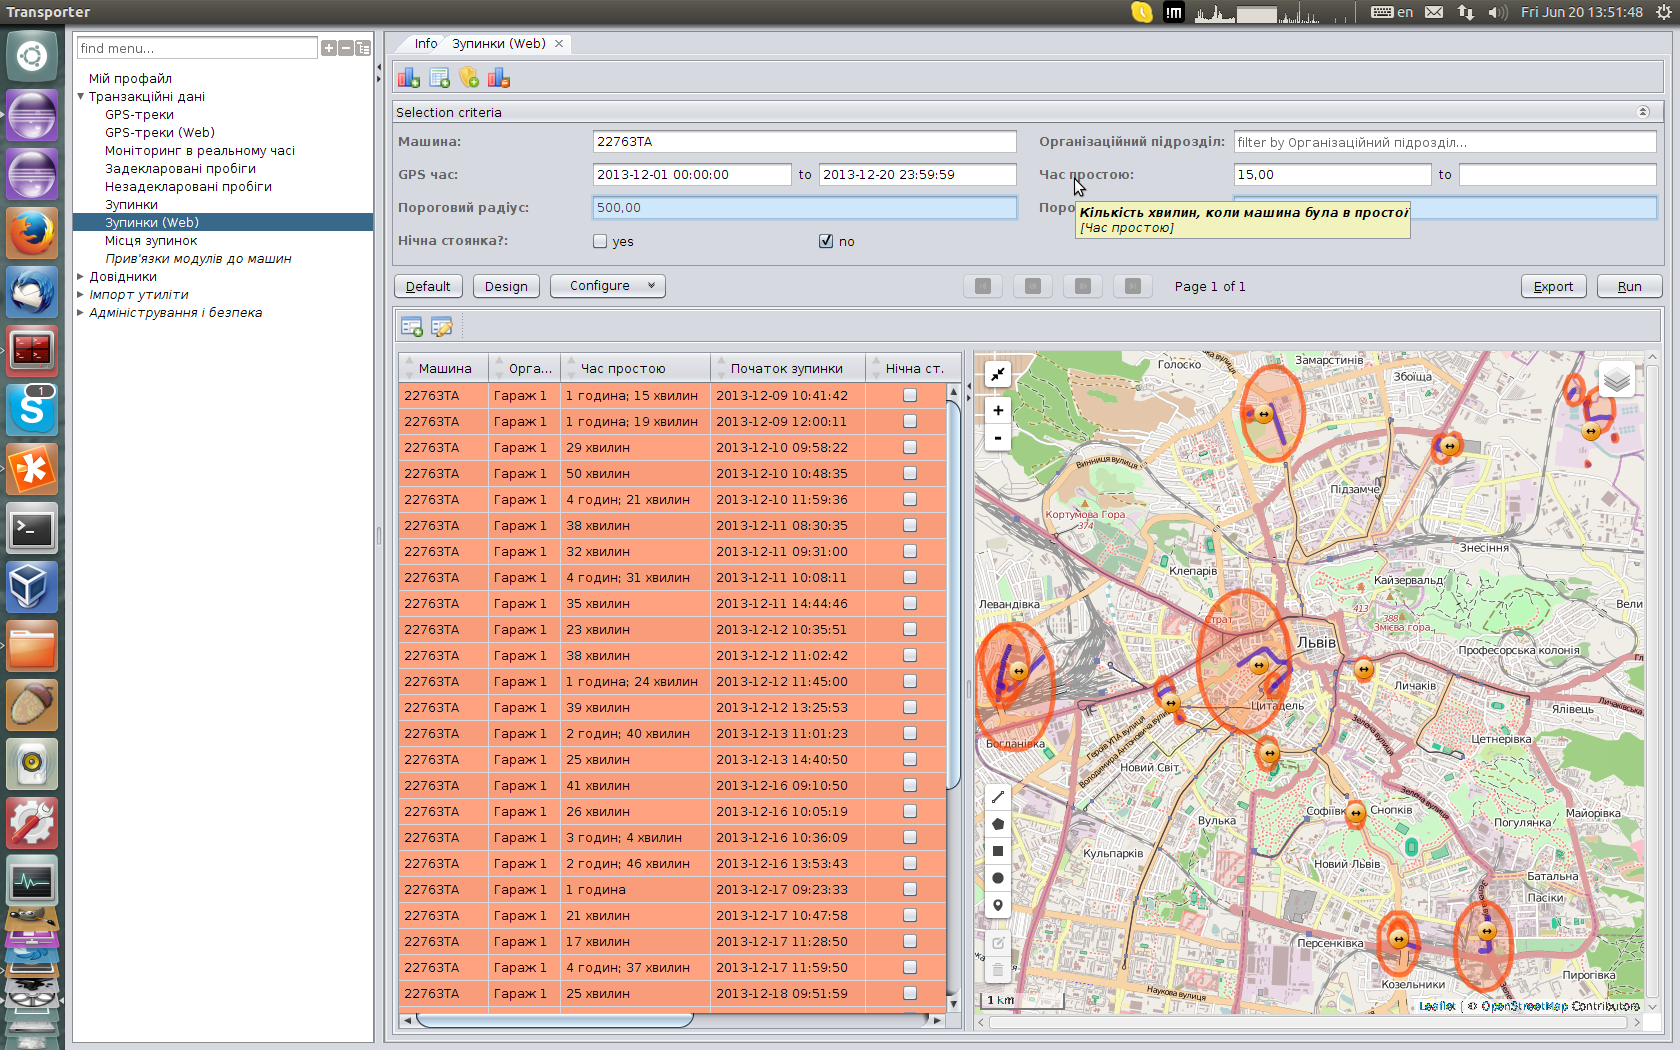
\includegraphics[width=\linewidth]{chapters/03-stoppages/images/27-determining-stoppages-with-more-than-15-minutes-duration.png}
\caption{Determining stoppages with more than 15 minutes duration}\label{fig:27}
\end{figure}